\section[The Baby]{
    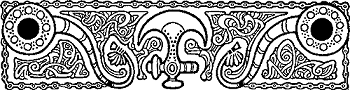
\includegraphics[width=9.3cm]{viking-tales/009}\\
    The Baby}

\lettrine{K}{ing Halfdan} lived in Norway long ago. One morning his
queen said to him:
\vskip\baselineskip
``I had a strange dream last night. I thought that I stood in the grass
before my bower.\footnote{See note about house on page~\pageref{house}.}
I pulled a thorn from my dress. As I held it in my fingers, it grew into
a tall tree. The trunk was thick and red as blood, but the lower limbs
were fair and green, and the highest ones were white. I thought that the
branches of this great tree spread so far that they covered all Norway
and even more.''

``A strange dream,'' said King Halfdan. ``Dreams are the messengers of
the gods. I wonder what they would tell us,'' and he stroked his beard
in thought.

Some time after that a serving-woman came into the feast hall where King
Halfdan was. She carried a little white bundle in her arms.

``My lord,'' she said, ``a little son is just born to you.''

``Ha!'' cried the king, and he jumped up from the high seat and hastened
forward until he stood before the woman.

``Show him to me!'' he shouted, and there was joy in his voice.

The serving-woman put down her bundle on the ground and turned back the
cloth. There was a little naked baby. The king looked at it carefully.

``It is a goodly youngster,'' he said, and smiled. ``Bring Ivar and
Thorstein.''\footnote{See note about names on page~\pageref{names}.}

They were captains of the king's soldiers. Soon they came.

``Stand as witnesses,'' Halfdan said.

Then he lifted the baby in his arms, while the old serving-woman brought
a silver bowl of water. The king dipped his hand into it and sprinkled
the baby, saying:

``I own this baby for my son. He shall be called Harald. My naming gift
to him is ten pounds of gold.''

Then the woman carried the baby back to the queen's room.

\begin{figure}
    \centering
    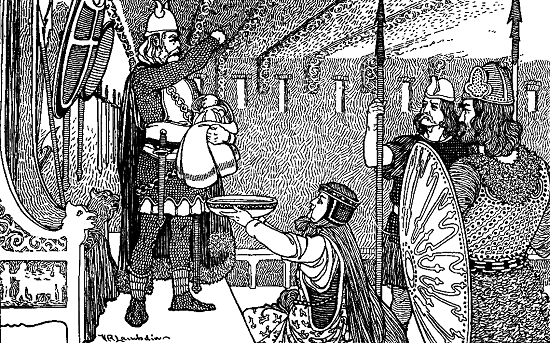
\includegraphics[width=14.6cm]{viking-tales/010}
    \caption{``I own this baby for my son. He shall be called Harald''}
\end{figure}

``My lord owns him for his son,'' she said. ``And no wonder! He is
perfect in every limb.''

The queen looked at him and smiled and remembered her dream and thought:

``That great tree! Can it be this little baby of mine?''

\begin{figure}[hb]
    \centering
    \vskip8pt
    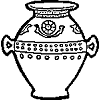
\includegraphics[width=2.7cm]{viking-tales/011}
\end{figure}
